\subsection{Class Diagram}


\begin{figure}[h!]
\centering
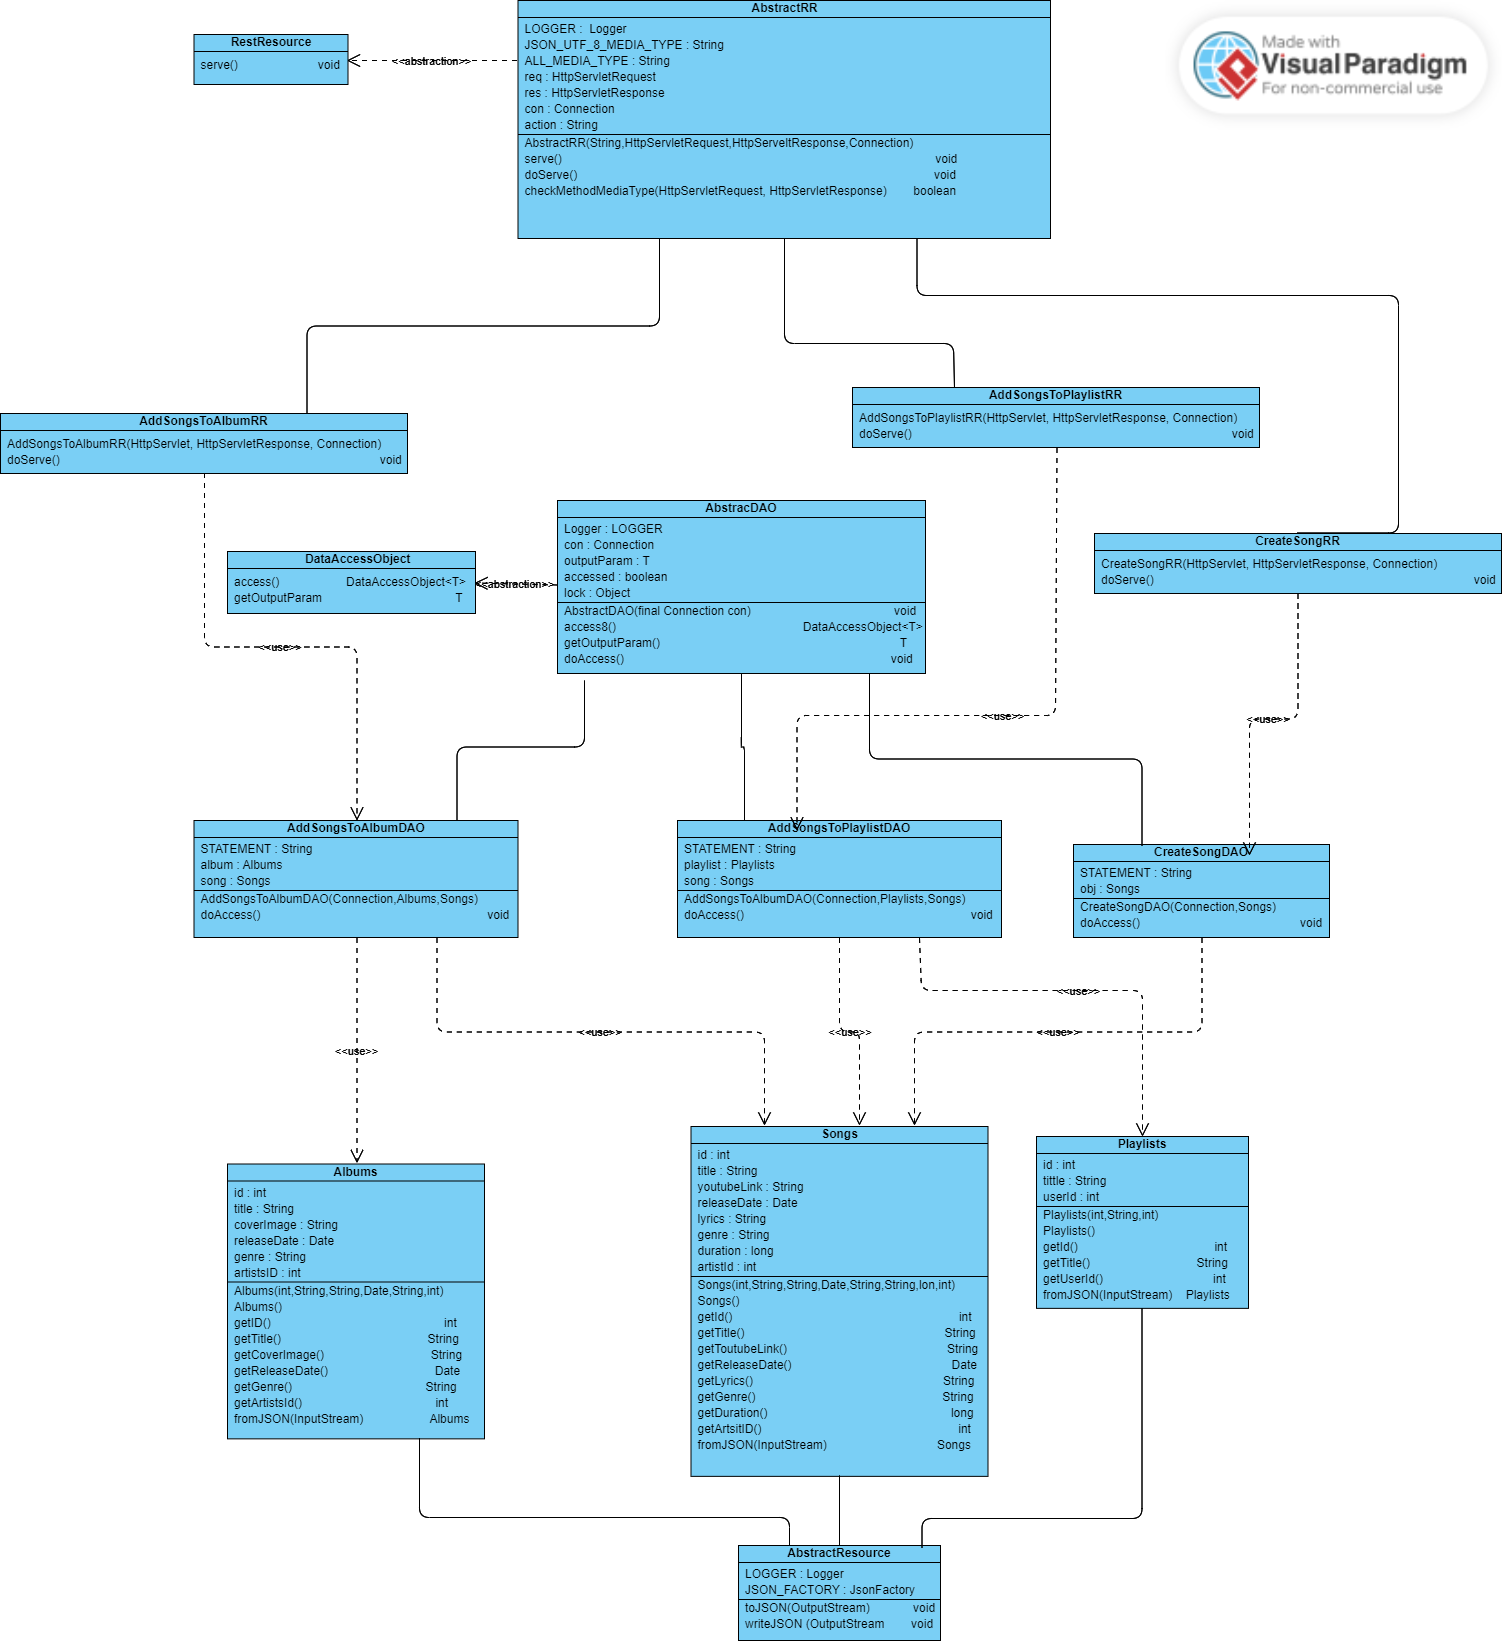
\includegraphics[width=0.9\textwidth]{sections/BLL/classdiagram.png}
\caption{Class Diagram}
\end{figure}

%Describe here the class diagram of your project

The class diagram contains (some of) the classes used to handle three types of resources: songs, albums and playlists. It is possible to observe that we have REST classes to handle all of the actions we are showing in the diagram. Each REST extends the AbstractRR which is needed to acquire the connection to the database. All of the RR classes implement the method doServe() and parse the URI, determining the type of resource the user wants to interact with.

The RR files also call the corresponding Data Access Objects (DAOs) that allows us to obtain different resources. We have one DAO for each RR file.

Concerning the Songs, in this diagram we have three REST classes that are: \verb|AddSongsToAlbumsRR|, \\
\verb|AddSongsToPlaylistsRR| and \verb|CreateSongsRR|, all of them extend the class \verb|AbstractRR| that implements the interface \verb|RestResource|. All of the RR files implements in their operations the corresponding DAO, in this case we have \verb|AddSongsToAlbumsDAO|, \verb|AddSongsToPlaylistsDAO| and \verb|CreateSongsDAO|. All the DAO files extend the class \verb|AbstractDAO| that implements the interface \verb|DataAccessObject|.
The rest of the classes have a similar structure. Overall, this design allows for separation of logic paths, with REST classes handling HTTP communication and DAOs handling database operations.

%The class diagram contains (some of) the classes used to handle five types of resources: users, songs, albums, playlist and artists. It is possible to observe that we have REST classes to handle every possible action. Each REST extends the AbstractRR which is needed to acquire the connection to the database. All of them implement the method doServe() and parse the URI.

%Concerning the Users, there are multiple REST classes used to handle the user resource. In particular we have CreateUserRR, that creates a user; DeleteUserRR that eliminates a user from the database; InfoUserRR that shows the information of the user; and UpdateUserRR that update the data of the selected user.

%Concerning the Songs, there a lot of REST classes in order to handle the song resource. Similar to the previous ones, we have CreateSongRR, DeleteSongRR, InfoSongRR. As new REST classes we have AddSongsToAlbumRR and AddSongsToPlaylistRR that add the song in a speficic album or playlist, DeleteSongFromPlaylistRR that deletes a song from a playlist and the ListSongsByArtistRR and ListSongsByAlbumRR, that make list of the songs searched by its artists or album. We also have UnlikeSongRR that unlikes a song from the user profile.

%Concerning the Albums, there are many REST classes in order to manage the artists resource. Practicaly identical to the previous ones, we have CreateAlbumRR, DeleteAlbumRR, InfoAlbumRR, LikeAlbumRR, UnlikeAlbumRR and the listing part that are: ListAlbumsByArtistsRR and ListAlbumsLikedByUsersRR.

%Concerning to the Playlist class, there a multiple REST classes similar to the ones before, that help handling the playlist resource.
%Concerning to the Artist class, the REST classes are equivalent to the ones in the User part.




